\chapter{Il progetto di stage}
\label{cap:descrizione-stage}

\intro{In questo capitolo viene descritto nel dettaglio il progetto includendo gli obiettivi richiesti e la pianificazione del lavoro per la sua realizzazione. Infine viene motivata la scelta di tale progetto.}

\section{Descrizione del progetto}
\label{sec:descrizione-progetto}

Lo scopo del progetto di stage è quello di sviluppare un'applicazione \gls{crossplatform}\glsoccur per la gestione di \gls{meetingnote}\glsoccur e relativa documentazione.
Nello specifico, l'applicazione deve fornire le seguenti funzionalità:
\begin{itemize}
    \item \textbf{creazione} di una \gls{meetingnote}\glsoccur, inserendo le informazioni richieste, essa può avvenire in due modi:
    \begin{itemize}
        \item inserimento \textbf{manuale} dei dati attraverso un \gls{wizard}\glsoccur di creazione;
        \item integrazione con \gls{openai}\glsoccur per \textbf{automatizzare} il processo di creazione.
    \end{itemize}
    \item possibilità di \textbf{modificare} una \gls{meetingnote}\glsoccur già creata, attraverso un \gls{wizard}\glsoccur di modifica, analogo a quello di creazione;
    \item possibilità di \textbf{eliminare} una \gls{meetingnote}\glsoccur dalla lista di quelle create;
    \item \textbf{visualizzazione} di una lista di \gls{meetingnote}\glsoccur, con la possibilità di filtrarla per \gls{cliente}\glsoccur, data e ordine di creazione (dalla più recente o meno recente), inoltre, per ciascuna, è possibile visualizzarne in dettaglio il contenuto;
    \item integrazione con il sistema di \textbf{autenticazione} della piattaforma \emph{RiskAPP}, essa può avvenire in due modalità differenti:
    \begin{itemize}
        \item inserimento \textbf{manuale} delle credenziali;
        \item tramite \textbf{\gls{riconoscimentobiometrico}}\glsoccur.
    \end{itemize}
    \item possibilità di visualizzare i \textbf{dati dell'utente}.
\end{itemize}

\section{Obiettivi}
\label{sec:obiettivi}

In questa sezione verranno illustrati gli obiettivi, definiti nel \emph{Piano di Lavoro}, che si prevede di raggiungere durante lo svolgimento del progetto di stage.

\subsection{Notazione}
\label{subsec:notazione}

Si farà riferimento alla seguente notazione per indicare il grado di importanza degli obiettivi fissati:
\begin{itemize}
    \item \textbf{O}, identifica i requisiti obbligatori, vincolanti in quanto obiettivo primario richiesto dal committente;
    \item \textbf{D}, identifica i requisiti desiderabili, non vincolanti o strettamente necessari, ma dal riconoscibile valore aggiunto;
    \item \textbf{F}, identifica i requisiti facoltativi, rappresentanti valore aggiunto non strettamente competitivo.
\end{itemize}
Le sigle indicate saranno seguite da una coppia sequenziale di numeri, che identificano univocamente ogni obiettivo.

\subsection{Obiettivi fissati}
\label{subsec:obiettivi-fissati}

Si prevede lo svolgimento dei seguenti obiettivi:
\begin{itemize}
    \item \textbf{Obbligatori}
    \begin{itemize}
        \item \textbf{O01}\label{O01}: implementare un meccanismo di autenticazione attraverso delle chiamate all'\gls{apig}\glsoccur della piattaforma \emph{RiskAPP};
        \item \textbf{O02}\label{O02}: richiamare, attraverso richieste \gls{httpg}\glsoccur, le \gls{apig}\glsoccur per ottenere i dati necessari da visualizzare;
        \item \textbf{O03}\label{O03}: creazione delle \gls{meetingnote}\glsoccur;
        \item \textbf{O04}\label{O04}: compilazione del contenuto delle \gls{meetingnote}\glsoccur in maniera testuale e vocale;
        \item \textbf{O05}\label{O05}: sviluppo della \gls{uig}\glsoccur grafica dell'applicazione;
    \end{itemize}
    \item \textbf{Desiderabili}
    \begin{itemize}
        \item \textbf{D01}\label{D01}: integrazione di \gls{openai}\glsoccur per la creazione automatica delle \gls{meetingnote}\glsoccur;
        \item \textbf{D02}\label{D02}: \gls{deploy}\glsoccur dell'applicazione sulle piattaforme \emph{Android} e \emph{iOS};
    \end{itemize}
    \item \textbf{Facoltativi}
    \begin{itemize}
        \item \textbf{F01}\label{F01}: implementazione dei test per la verifica e validazione dell'applicazione;
    \end{itemize}
\end{itemize}

\section{Pianificazione}
\label{sec:pianificazione}

Di seguito viene riportata la pianificazione delle attività da svolgere durante il periodo di stage, suddivise per settimane.

\subsection{Pianificazione iniziale}
\label{subsec:pianificazione-iniziale}

In questa sezione viene riportata la pianificazione iniziale, definita anteriormente al periodo di stage, documentata nel \emph{Piano di Lavoro}, e il preventivo della durata delle attività, nella Tabella \ref{tab:preventivo-ore} , espresso in ore, che si prevede di impiegare per la realizzazione del progetto di stage. \\

\subsubsection{Prima settimana: 24/07/23 - 28/07/23 (40 ore)}
    \begin{itemize}
        \item Incontro con il tutor aziendale per la presentazione dettagliata del progetto e comprensione dei requisiti richiesti;
        \item Visione del \emph{Tool trattative} e delle \gls{apig}\glsoccur, per la comprensione del contesto applicativo;
        \item Formazione sulle tecnologie e strumenti da utilizzare: \emph{Dart} \cite{site:dart}.
    \end{itemize}
\subsubsection{Seconda settimana: 31/07/23 - 04/08/23 (40 ore)}
    \begin{itemize}
        \item Formazione sulle tecnologie e strumenti da utilizzare: \emph{Figma} \cite{site:figma} e \emph{Flutter} \cite{site:flutter}.
    \end{itemize}
\subsubsection{Terza settimana: 07/08/23 - 11/08/23 (40 ore)}
    \begin{itemize}
        \item Realizzazione del \gls{mockup} dell'applicazione;
        \item Analisi dei requisiti;
        \item Fase di progettazione dell'applicazione e realizzazione del diagramma UML delle classi;
        \item Stesura della documentazione relativa alle attività di analisi dei requisiti e progettazione.
    \end{itemize}
\subsubsection{Quarta settimana: 14/08/23 - 18/08/23 (40 ore)}
    \begin{itemize}
        \item Inizio sviluppo dell'interfaccia utente (\gls{uig}\glsoccur) dell'applicazione (\textbf{O05});
        \item Implementazione del meccanismo di autenticazione (\textbf{O01});
        \item Chiamate alle \gls{apig}\glsoccur per ottenere i dati necessari da visualizzare (\textbf{O02});
        \item Stesura dei test per le funzionalità implementate (\textbf{F01}).
    \end{itemize}
\subsubsection{Quinta settimana: 21/08/23 - 25/08/23 (40 ore)}
    \begin{itemize}
        \item Implementazione della funzionalità di creazione delle \gls{meetingnote}\glsoccur (\textbf{O03});
        \item Implementazione della funzionalità di compilazione delle \gls{meetingnote}\glsoccur (\textbf{O04});
        \item Stesura dei test per le funzionalità implementate (\textbf{F01}).
    \end{itemize}
\subsubsection{Sesta settimana: 28/08/23 - 01/09/23 (40 ore)}
    \begin{itemize}
        \item Continuazione sviluppo \gls{uig}\glsoccur dell'applicazione (\textbf{O05});
        \item Integrazione di \gls{openai}\glsoccur per la creazione automatica delle \gls{meetingnote}\glsoccur (\textbf{D01}).
    \end{itemize}
\subsubsection{Settima settimana: 04/09/23 - 08/09/23 (40 ore)}
    \begin{itemize}
        \item Completamento dello sviluppo \gls{uig}\glsoccur dell'applicazione (\textbf{O05});
        \item Stesura dei test per le funzionalità implementate (\textbf{F01}).
    \end{itemize} 
\subsubsection{Ottava settimana: 11/09/23 - 15/09/23 (40 ore)}
    \begin{itemize}
        \item Esecuzione dei test per la verifica e validazione dell'applicazione (\textbf{F01});
        \item Stesura della documentazione relativa alle attività di codifica;
        \item \Gls{deploy}\glsoccur dell'applicazione sulle piattaforme \emph{Android} e \emph{iOS} (\textbf{D02}).
    \end{itemize}

    \begin{table}
        \centering
        \begin{tabularx}{\textwidth}{|c|X|}
            \hline
            \textbf{Ore pianificate} & \textbf{Descrizione dell'attività} \\\hline
            
            \textbf{80} & \textbf{Formazione sulle tecnologie} \\	 
            \hline
            
            \textbf{40} & \textbf{Definizione architettura di riferimento e relativa documentazione} \\ \hdashline 
            \multirow{3}{0cm}\\ 
            \textit{12} & 
            \textit{Analisi del problema e del dominio applicativo} \\
            \textit{22} & 
            \textit{Progettazione della piattaforma e relativi test} \\
            \textit{6} & 
            \textit{Stesura documentazione relativa ad analisi e progettazione} \\
            \hline
            
    
            \textbf{160} & \textbf{Sviluppo}  \\ \hdashline 
            \multirow{5}{0cm}\\ 
            \textit{26} & 
            \textit{Implementazione del meccanismo di autenticazione e integrazione con il sistema preesistente per il prelevamento dei dati da visualizzare nell'applicazione} \\
            \textit{34} & 
            \textit{Implementazione delle funzionalità di creazione e compilazione (testuale e vocale) delle meeting-note} \\
            \textit{28} & 
            \textit{Integrazione del servizio OpenAI} \\
            \textit{40} & 
            \textit{Attività di testing} \\
            \textit{32} & 
            \textit{Sviluppo UI} \\
            \hline
            
            \textbf{40} & \textbf{Verifica e Validazione finale}  \\ \hdashline 
            \multirow{3}{0cm}\\ 
            \textit{24} & 
            \textit{Esecuzione dei test per la verifica e collaudo dell'applicazione} \\
            \textit{8} & 
            \textit{Stesura documentazione finale} \\
            \textit{8} & 
            \textit{Deploy dell'applicazione} \\
            \hline
            
            \textbf{Totale ore} & \multicolumn{1}{|c|}{\textbf{320}} \\ 
            \hline
            
        \end{tabularx}
        \caption{Preventivo della durata delle attività}
        \label{tab:preventivo-ore}
    \end{table}

\subsection{Variazioni nella pianificazione}
\label{subsec:variazione-pianificazione}

Durante la prima settimana di stage, la pianificazione iniziale è stata subito non rispettata, questo però non ha compromesso negativamente in alcun modo il percorso di realizzazione del prodotto e il raggiungimento degli obiettivi fissati.\\
Una prima motivazione di tali variazioni è dettata da un consiglio del tutor aziendale di sviluppare un \gls{mockup}\glsoccur dell'applicazione, in modo da fornire un notevole aiuto nell'analisi dei requisiti e di conseguenza avere un'idea più chiara di come essa dovrà essere progettata e sviluppata.\\
Inoltre un'altra motivazione, è stata la mia esperienza pregressa, da autodidatta, con il linguaggio \emph{Dart} \cite{site:dart} e il framework \emph{Flutter} \cite{site:flutter}, che mi ha permesso saltare parzialmente parte della fase formativa.\\
Di seguito verranno riportate tali variazioni, visualizzabili anche nel diagramma di Gantt in Figura \ref{fig:gantt}, che corrispondono dunque all'effettivo svolgimento delle attività durante il periodo di stage, il cui consuntivo delle ore corrispondente è riportato nella Sezione \ref{sec:consultivo-attivita}.

\subsubsection{Prima settimana: 24/07/23 - 28/07/23 (40 ore)}
    \begin{itemize}
        \item Incontro con il tutor aziendale per la presentazione dettagliata del progetto e comprensione dei requisiti richiesti;
        \item Visione del \emph{Tool trattative} e delle \gls{apig}\glsoccur, per la comprensione del contesto applicativo;
        \item Formazione sulle tecnologie e strumenti da utilizzare: \emph{Figma} \cite{site:figma}.
        \item Realizzazione del \gls{mockup}\glsoccur dell'applicazione.
        \item Iniziata la fase di analisi dei requisiti dell'applicazione;
    \end{itemize}
\subsubsection{Seconda settimana: 31/07/23 - 04/08/23 (40 ore)}
    \begin{itemize}
        \item Completamento della fase di analisi dei requisiti dell'applicazione;
        \item Formazione sulle tecnologie e strumenti da utilizzare: \emph{Dart} \cite{site:dart} e \emph{Flutter} \cite{site:flutter};
        \item Iniziato sviluppo  della \gls{uig}\glsoccur dell'applicazione (\textbf{O05}).
    \end{itemize}
\subsubsection{Terza settimana: 07/08/23 - 11/08/23 (40 ore)}
    \begin{itemize}
        \item Completamento dello sviluppo della \gls{uig}\glsoccur dell'applicazione (\textbf{O05});
        \item Fase di progettazione dell'applicazione: ricerca e scelta del \gls{patternarchitetturale}\glsoccur e realizzazione del diagramma UML delle classi;
        \item Iniziato lo sviluppo del meccanismo di autenticazione: inserimento manuale delle credenziali (\textbf{O01});
    \end{itemize}
\subsubsection{Quarta settimana: 14/08/23 - 18/08/23 (32 ore)}
    \begin{itemize}
        \item Completamento dello sviluppo del meccanismo di autenticazione: inserimento manuale delle
        credenziali (\textbf{O01});
        \item Completamento delle funzionalità di ottenimento dei dati da visualizzare attraverso le \gls{apig}\glsoccur (\textbf{O02});
    \end{itemize}
\subsubsection{Quinta settimana: 21/08/23 - 25/08/23 (40 ore)}
    \begin{itemize}
        \item Completamento dello sviluppo della funzionalità di creazione e modifica delle \gls{meetingnote}\glsoccur (\textbf{O03});
        \item Completamento dello sviluppo della funzionalità di compilazione delle \gls{meetingnote}\glsoccur (\textbf{O04});
    \end{itemize}
\subsubsection{Sesta settimana: 28/08/23 - 01/09/23 (40 ore)}
    \begin{itemize}
        \item Completamento dello sviluppo del meccanismo di autenticazione: \gls{riconoscimentobiometrico} (\textbf{O01});
        \item Apportati miglioramenti della \gls{uig}\glsoccur per l'ottimizzazione dell'esperienza utente;
        \item Effettuate ottimizzazioni per le performance e refactoring del codice;
    \end{itemize}
\subsubsection{Settima settimana: 04/09/23 - 08/09/23 (40 ore)}
    \begin{itemize}
        \item Impostazione icona e nome dell'applicazione;
        \item Apportati miglioramenti e ottimizzazione del codice;
        \item Commentato il codice e redatta la documentazione relativa alle attività di sviluppo;
        \item Completamento dello sviluppo della \gls{uig}\glsoccur delle viste riguardanti alla creazione automatica delle \gls{meetingnote}\glsoccur  (\textbf{O05});
    \end{itemize}
\subsubsection{Ottava settimana: 11/09/23 - 15/09/23 (40 ore)}
    \begin{itemize}
        \item Completamento dello sviluppo della funzionalità di creazione automatica delle \gls{meetingnote}\glsoccur (\textbf{D01});
        \item Aggiornamento della documentazione relativa alle attività di codifica;
        \item Apportati miglioramenti e ottimizzazione del codice;
    \end{itemize}

È doveroso precisare che, nonostante la fase di progettazione sia avvenuta dopo la codifica della \gls{uig}\glsoccur dell'applicazione e non vicerversa, come previsto nella pianificazione iniziale, ma soprattutto dai principi dell'\gls{ingsw}\glsoccur, non si è andati a compromettere la fase di sviluppo, in quanto la codifica della \gls{uig}\glsoccur si è svolta con la consapevolezza di implementare un'architettura che si basasse sul \gls{patternarchitetturale}\glsoccur \Gls{mvcg}\glsoccur, per mantenere una separazione tra la logica di presentazione e la logica di business.

\begin{figure}[!h] 
    \centering 
    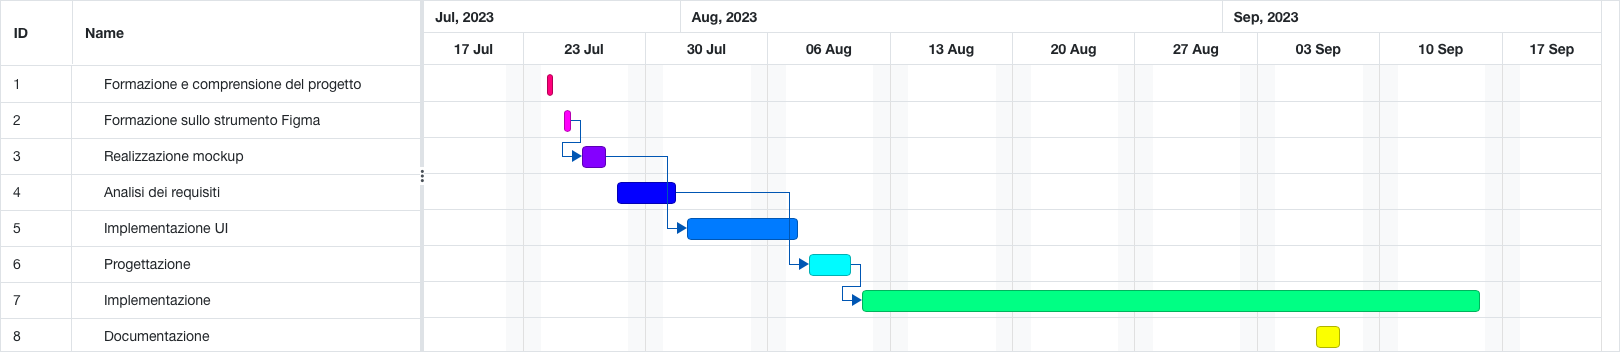
\includegraphics[width=1.0\columnwidth]{gantt_stage} 
    \caption{Diagramma di Gantt della ripartizione definitiva delle attività durante il periodo di stage}
    \label{fig:gantt}
\end{figure}

\section{Motivazione della scelta}
\label{sec:motivazione-scelta}

La scelta di tale progetto è stata dettata da varie motivazioni, alcune indipendenti da esso, ovvero la possibilità di mettersi in gioco e cercare di applicare le conoscenze acquisite durante il percorso di studi, in un contesto più professionale e reale. \\
Inoltre, come menzionato in precedenza, la mia esperienza pregressa con le tecnologie impiegate, mi ha semplificato la decisione, in quanto avere avuto la possibilità di utilizzarle per sviluppare un progetto in un contesto lavorativo è stato stimolante e gratificante, nonostante mi abbia anche permesso di saltare parzialmente la fase formativa, è stata comunque necessaria per approfondire le conoscenze e acquisirne di nuove.
